\documentclass{beamer}

\usepackage{listings}
\usepackage{xcolor}
\usepackage{graphicx}

\definecolor{codegreen}{rgb}{0,0.6,0}
\definecolor{codegray}{rgb}{0.5,0.5,0.5}
\definecolor{codepurple}{rgb}{0.58,0,0.82}
\definecolor{backcolour}{rgb}{0.95,0.95,0.92}

\lstdefinestyle{mystyle}{
    backgroundcolor=\color{backcolour},   
    commentstyle=\color{codegreen},
    keywordstyle=\color{magenta},
    numberstyle=\tiny\color{codegray},
    stringstyle=\color{codepurple},
    basicstyle=\ttfamily\footnotesize,
    breakatwhitespace=false,         
    breaklines=true,                 
    captionpos=b,                    
    keepspaces=true,                 
    numbers=left,                    
    numbersep=5pt,                  
    showspaces=false,                
    showstringspaces=false,
    showtabs=false,                  
    tabsize=2
}

\lstset{style=mystyle}

%Information to be included in the title page:
\title{Low Level AVR}
\subtitle{Arduino? Nein danke!}
\author{Felix Queißner}
\institute{shackspace}
\date{2020}

\begin{document}

\frame{\titlepage}

\begin{frame}
\frametitle{Wer bin ich?}
\begin{itemize}
\item Felix „xq“ Queißner
\item Baujahr 1993
\item Mit 12 angefangen, zu programmieren
\item Mit 13 angefangen, Elektronik zu basteln
\item Mache gerne Dinge mit Code und alten Computern
\end{itemize}
\end{frame}

\begin{frame}
\frametitle{Worum geht's?}
\begin{itemize}
\item Grundlagenwissen AVR-Programmierung vermitteln
\item „Wie komme ich klar, wenn es mit der Arduino-IDE nicht mehr weiter geht?“
\item „Awareness schaffen“ für Code Bloat
\item \textbf{Nicht:} AVR/Arduino löten
\item \textbf{Nicht:} C programmieren lernen
\end{itemize}
\end{frame}

\begin{frame}
\frametitle{Outline}
\begin{enumerate}
\item Teaser
\item The Arduino way
\item Zum Ziel in vier Schritten
  \begin{enumerate}
  \item Dokumentation lesen
  \item Code schreiben
  \item Compilen \& Linken
  \item Flashen
  \end{enumerate}
\item Fazit
\item Wie geht's weiter?
\end{enumerate}
\end{frame}

\begin{frame}
\frametitle{Wie kommen wir von hier …}
\lstinputlisting[language=C]{bad-code.c}
\end{frame}

\begin{frame}
\frametitle{… nach da?}
\lstinputlisting[language=C]{good-code.c}
\end{frame}

\begin{frame}
\frametitle{The Arduino way}
\begin{itemize}
\item Schnell von „Idee“ zu „Es blinkt schon mal was“ kommen
\item Single-Click-Solution
\item Mit was man genau arbeitet ist eigentlich egal, es erfüllt alles den gleichen Zweck 
\end{itemize}
\end{frame}

\begin{frame}
\frametitle{Blink}
\begin{itemize}
\item Lässt eine LED mit \(\frac{1}{2}\) Hertz blinken
\item Benutzt \lstinline[language=C]{setup()} und \lstinline[language=C]{loop()}
\end{itemize}
\lstinputlisting[language=C]{blink.ino}
\end{frame}

\begin{frame}
\frametitle{Serial}
\begin{itemize}
\item Gibt \lstinline[language=C]{"Hello, World!"} auf der Konsole aus
\item Spiegelt anschließend die Texteingabe zurück
\item Benutzt \lstinline[language=C]{setup()} und \lstinline[language=C]{loop()}
\item Benutzt \lstinline[language=C]{Serial.*}
\end{itemize}
\lstinputlisting[language=C]{serial.ino}
\end{frame}

\begin{frame}
\frametitle{Pro/Contra Arduino}

\textbf{Pro:}
\begin{itemize}
\item Man kommt schnell zum Ziel
\item Zugrunde liegened Hardware ist schnell ausgetauscht
\item Es gibt viele Beispiele für die Arduino-Welt
\item „Batterien inklusive“
\end{itemize}

\textbf{Contra:}
\begin{itemize}
\item Es passiert sehr viel \textit{Magie}
\item Arduino-Programme sind „fett und träge“
\item Wir haben keine wirkliche Kontrolle über das Programm
\end{itemize}
  
\end{frame}

\begin{frame}
\frametitle{In vier Schritten zum Ziel}
\begin{enumerate}
\item Dokumentation lesen
\item Code schreiben
\item Compilen \& Linken
\item Flashen
\end{enumerate}
\end{frame}

\begin{frame}
\frametitle{Warum tun wir uns das an?}
\begin{itemize}
\item Programme werden kleiner
\item Programme werden schneller
\item Wir können die Hardware voll ausnutzen
\end{itemize}
\end{frame}

\begin{frame}
\frametitle{Schritt 1: Dokumentation lesen}

\textbf{Welche Dokumente brauchen wir?}
\begin{itemize}
\item Schaltplan
\item Datenblatt
\end{itemize}
\end{frame}

\begin{frame}
\frametitle{Schaltplan}
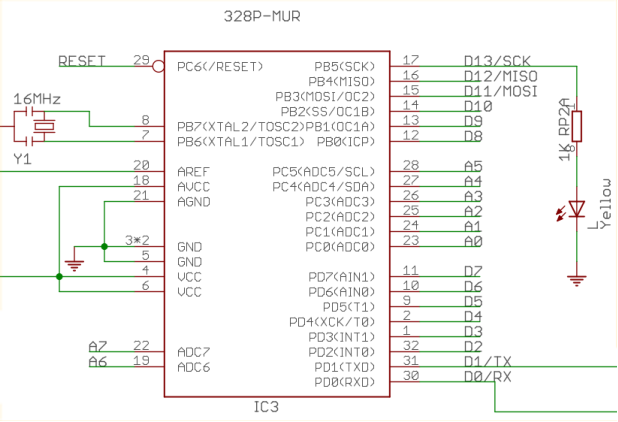
\includegraphics{schematic.pdf}
\end{frame}

% PC6 ist Reset, aber auch I/O!

\begin{frame}
\frametitle{Schaltplan}
\begin{itemize}
\item \textit{Ground Truth} für Pinbelegungen
\item Zeigt uns, wie die Hardware funktioniert
\item Offenbart manchmal undokumentierte Möglichkeiten
\end{itemize}


\end{frame}


% D6, D7 können als Input für den Analog-Komparator dienen!
% D2, D3 können externe Interrupts!

\begin{frame}
\frametitle{Datenblatt}
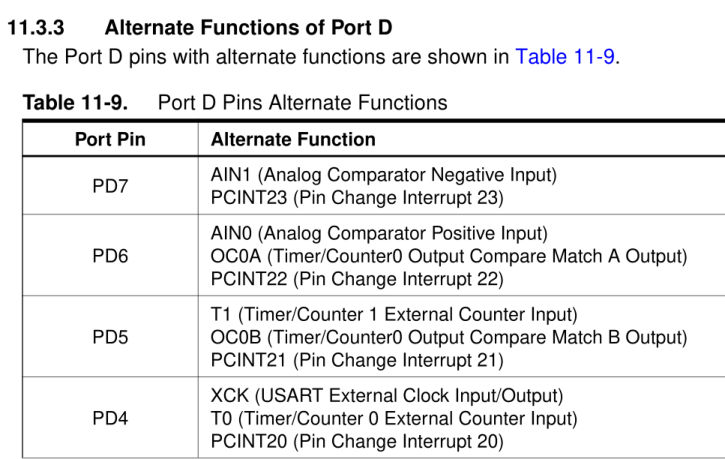
\includegraphics{datasheet.pdf}
\end{frame}

\begin{frame}
\frametitle{Datenblatt}
\begin{itemize}
\item \textit{Ground Truth} für Hardware-Funktionalität
\item Zeigt uns, wie der Microcontroller funktioniert
\item Hilfreich: Doppelfunktionen für Pin-Belegungen
\end{itemize}

\end{frame}

\begin{frame}
\frametitle{Schritt 2: Code schreiben}

\textbf{Allgemein:}
\begin{itemize}
\item C ist die primäre Embedded-Programmiersprache
\item C++, Basic, Pascal, Zig, Rust, … sind auf AVR ebenfalls verfügbar
\item Dynamische Speicherverwaltung wird selten benötigt
\end{itemize}

\textbf{Hands on:}
\begin{enumerate}
\item Code
\item Datenblatt verwenden
\item Komplexer Hardware-Init
\item Interrupt
\end{enumerate}
\end{frame}

\begin{frame}
\frametitle{Hands on: Code (Blink 1)}
\lstinputlisting[language=C]{blink1.c}
\end{frame}

\begin{frame}
\frametitle{Hands on: Datenblatt (Blink 2)}
\lstinputlisting[language=C]{blink2.c}
\end{frame}

\begin{frame}
\frametitle{Hands on: Hardware-Init (UART 1)}
\lstinputlisting[language=C]{uart1.c}
\end{frame}

\begin{frame}
\frametitle{Hands on: Interrupts (UART 2)}
\lstinputlisting[language=C]{uart2.c}
\end{frame}

\begin{frame}
\frametitle{Schritt 3: Compilen \& Linken}
- Was ist ein
    - Compiler?
    - Linker?
    - Bibliothek?
    - Makefile?
- Dateiformate
- Tools
\end{frame}

\begin{frame}
\frametitle{Was ist ein Compiler?}
\end{frame}

\begin{frame}
\frametitle{Was ist ein Linker?}
\end{frame}

\begin{frame}
\frametitle{Was ist eine Bibliothek?}
\end{frame}

\begin{frame}
\frametitle{Was ist ein Makefile?}
\end{frame}

\begin{frame}
\frametitle{Dateiformate}
- Dateiformate
    - elf object
    - elf executable
    - ihex
\end{frame}

\begin{frame}
\frametitle{Tools}
    - objdump
    - size
    - addr2line
\end{frame}

\begin{frame}
\frametitle{objdump}
\end{frame}

\begin{frame}
\frametitle{size}
\end{frame}

\begin{frame}
\frametitle{addr2line}
\end{frame}

\begin{frame}
\frametitle{Schritt 4: Flashen}
- Möglichkeiten
    - High Voltage Serial Programming 
    - In-System Programming
    - Bootloader
- Tools
  - avrdude
  - PonyProg
  - AVRStudio
  - …
\end{frame}

\begin{frame}
\frametitle{In-System Programming}
\end{frame}

\begin{frame}
\frametitle{Bootloader}
\end{frame}

\begin{frame}
\frametitle{avrdude}
\end{frame}

\begin{frame}
\frametitle{Was haben wir gewonnen?}
\begin{itemize}
\item Wir haben die Kontrolle über den Code
\item Wir können die Hardware voll ausnutzen
\item Unsere Programme sind kleiner
\item Unsere Programme benötigen weniger CPU-Zeit
\end{itemize}
\end{frame}

\begin{frame}
\frametitle{Vergleich: Blink}
\end{frame}

\begin{frame}
\frametitle{Vergleich: Serial}
\end{frame}

\begin{frame}
\frametitle{Wie geht's weiter?}

\textbf{Programmierung:}
\begin{itemize}
\item C++
\item Bibliotheken
\end{itemize}

\textbf{Links:}
\begin{itemize}
\item mikrocontroller.net
\item Roboternetz.de
\item Quellcode aus den Slides\\https://github.com/MasterQ32/avr-tutorial
\end{itemize}
\end{frame}

\begin{frame}
\frametitle{}
\begin{center}
\Huge{\textbf{Fragen?}}
\end{center}
\end{frame}

\end{document}